\subsection{Dirac Operator}
\label{sec:dirac}

The Dirac operator is the kernel routine of any lattice QCD
application, because its inverse is needed for the HMC update
procedure and also for computing correlation functions. The inversion
is usually performed by means of iterative solvers, like the conjugate
gradient algorithm, and hence the repeated application of the Dirac
operator to a spinor field is needed. Thus the optimisation of this
routine deserves special attention.

At some space-time point $x$ the application of a Wilson type Dirac
operator is mainly given by
\begin{equation}
  \label{eq:Dpsi}
  \begin{split}
    \phi(x) = & (m_0 + 4r +i\mu_q\gamma_5)\psi(x) \\
    &- \frac{1}{2}\sum_{\mu = 1}^4\Bigl[
    U_{x,\mu}(r+\gamma_\mu) \psi(x+a\hat\mu)  + U^\dagger_{x-a\hat\mu,\mu}
    (r-\gamma_\mu)\psi(x-a\hat\mu)\Bigr] \\
  \end{split}
\end{equation}
where $r$ is the Wilson parameter, which we set to one in the
following. The most computer time consuming part is the next-neighbour
interaction part.

For this part it is useful to observe that 
\[
(1\pm \gamma_\mu)\psi
\]
has only two independent spinor components, the other two follow
trivially. So only two of the components need to be computed, then
to be 
multiplied with the corresponding gauge field $U$, and then the other
two components are to be reconstructed.

The operation in eq.~(\ref{eq:Dpsi}) must be performed for each space-time
point $x$. If the loop over $x$ is performed such that all elements
of $\phi$ are accessed sequentially (one output stream), it is clear
that the elements in $\psi$ and $U$ cannot be accessed sequentially as
well. This non-sequential access may lead to serious performance
degradations due to too many cache misses, because modern processing
units have only a very limited number of input streams available. 

While the $\psi$  field is usually different from
one to the next application of the Dirac operator, the gauge field
stays often the same for a large number of applications. This is for
instance so in iterative solvers, where the Dirac operator is applied
$\mathcal{O}(1000)$ times with fixed gauge fields. Therefore it is
useful to construct a double copy of the original gauge field sorted
such that the elements are accessed exactly in the order needed in the
Dirac operator. For the price of additional memory, with this simple
change one can obtain large performance improvements, depending on the
architecture. The double copy must be updated whenever the gauge field
change. This feature is available in the code at configure time, the
relevant switch is {\ttfamily --with-gaugecopy}.

Above we were assuming that we run sequentially through the resulting
spinor field $\phi$. Another possibility is to run sequentially
through the source spinor field $\psi$. Moreover, one could split up
the operation (\ref{eq:Dpsi}) as follows, introducing intermediate
result vectors $\varphi^\pm$ with only two spinor components per lattice
site\footnote{We thank Peter Boyle for useful discussions on this
  point.}. Concentrating on the hopping part only, we would have 
\begin{equation}
  \label{eq:Dsplit}
  \begin{split}
    \varphi^+(x, \mu) &= P_{+\mu}^{4\to2}\ U_{x,\mu}(r+\gamma_\mu) \psi(x) \\
    \varphi^-(x, \mu) &= P_{-\mu}^{4\to2}\ (r-\gamma_\mu) \psi(x)\; . \\
  \end{split}
\end{equation}
From $\varphi^\pm$ we can then reconstruct the resulting spinor field 
as
\begin{equation}
  \label{eq:Dunsplit}
  \begin{split}
    \phi(x) =& \sum_\mu P_{+\mu}^{2\to4}\varphi^+(x+a\hat\mu,\mu) \\
    & + \sum_\mu P_{-\mu}^{2\to4}U^\dagger_{x-a\hat\mu,\mu}\varphi^-(x-a\hat\mu,\mu)
%    \phi(x-a\hat\mu) &= P_{+\mu}^{2\to4}\ \varphi^+(x, \mu) \\
%    \phi(x+a\hat\mu) &= P_{-\mu}^{2\to4}\
%    U^\dagger_{x-a\hat\mu,\mu}\varphi^-(x, \mu\; .)
  \end{split}
\end{equation}
Here we denote with $P_{\pm\mu}^{4\to2}$ the projection to the two
independent spinor components for $1\pm\gamma_\mu$ and with
$P_{\pm\mu}^{2\to4}$ the corresponding reconstruction.
The half spinor fields $\varphi^\pm$ can be interlaced in
memory such that $\psi(x)$ as well as $\varphi^\pm(x)$ are always
accessed sequentially in memory. The same is possible for the gauge
fields, as explained above. So only for $\phi$ we cannot avoid strided
access. So far we have only introduced extra fields $\varphi^\pm$,
which need to be loaded and stored from and to main memory, and
divided the Dirac operator into two steps (\ref{eq:Dsplit}) and
(\ref{eq:Dunsplit}) which are very balanced with regard to memory
bandwidth and floating point operations.

The advantage of this implementation of the Dirac operator comes
in the parallel case. In step (\ref{eq:Dsplit}) we need only elements
of $\psi(x)$, which are locally available on each node. So this step
can be performed without 
any communication. In between step (\ref{eq:Dsplit}) and
(\ref{eq:Dunsplit}) one then needs to communicate part of
$\varphi^\pm$, however only half the amount is needed compared to a
communication of $\psi$. After the second step there is then no
further communication needed. Hence, one can reduce the amount of data
to be send by a factor of two. 

There is yet another performance improvement possible with this form
of the Dirac operator, this time for the price of precision. One can
store the intermediate fields $\varphi^\pm$ with reduced precision,
e.g. in single precision when the regular spinor fields are in double
precision. This will lead to a result with reduced precision, however,
in a situation where this is not important, as for instance in the MD
update procedure, it reduces the data to be communicated by another
factor of two. And the required memory bandwidth is reduced as well.
This version of the hopping matrix (currently it is only implemented
for the hopping matrix) is available at configure time with the switch
{\ttfamily --enable-halfspinor}. 

The reduced precision version (sloppy precision) is available through
the input parameter {\ttfamily UseSloppyPrecision}. It will be used in
the MD update where appropriate. Moreover, it is implemented in the CG
iterative solver following the ideas outlined in
Ref.~\cite{Chiarappa:2006hz} for the overlap operator.

The various implementations of the Dirac operator can be found in the
file {\ttfamily D\_psi.c} and -- as needed for even/odd
preconditioning -- the hopping matrix in the file {\ttfamily
  Hopping\_Matrix.c}. There are many different versions of these two
routines available, each optimised for a particular architecture,
e.g. for the Blue Gene/P double hummer processor or the streaming SIMD
extensions of modern PC processors (SSE2 and SSE3), see also
Ref.~\cite{Luscher:2001tx}. Martin L{\"u}scher has made available his
standard C and SSE/SSE2 Dirac operator~\cite{Luscher:sse} under the
GNU General Public License, which are partly included into the tmLQCD
package.

\subsubsection{Blue Gene Version}

The IBM PowerPC 450d processor used on the Blue Gene architecture
provides a dual FPU, which supports a set of SIMD operations working
on 32 special registers useful for lattice QCD. These operations can
be accessed using build in functions of the IBM XLC compiler.
The file {\ttfamily bgl.h} contains all macros relevant for the Blue
Gene version of the hopping matrix and the Dirac operator. 

\begin{algorithm}[t]
  \caption{$\varphi^+ = \kappa\, U\, P_{+0}^{4\to2}(1+\gamma_0)\psi$}
  \begin{algorithmic}[1]
    \STATE // load components of $\psi$ into registers
    \STATE \_bgl\_load\_rs0((*s).s0);
    \STATE \_bgl\_load\_rs1((*s).s1);
    \STATE \_bgl\_load\_rs2((*s).s2);
    \STATE \_bgl\_load\_rs3((*s).s3);
    \STATE // prefetch gauge field for next direction $(1+\gamma_1)$
    \STATE \_prefetch\_su3(U+1);
    \STATE // do now first $P_{+0}^{4\to2}(1+\gamma_0)\psi$
    \STATE \_bgl\_vector\_add\_rs2\_to\_rs0\_reg0();
    \STATE \_bgl\_vector\_add\_rs3\_to\_rs1\_reg1();
    \STATE //now multiply both components at once with gauge field $U$ and $\kappa$
    \STATE \_bgl\_su3\_multiply\_double((*U));
    \STATE \_bgl\_vector\_cmplx\_mul\_double(ka0); 
    \STATE // store the result
    \STATE \_bgl\_store\_reg0\_up((*phi[ix]).s0);
    \STATE \_bgl\_store\_reg1\_up((*phi[ix]).s1);
  \end{algorithmic}
  \label{alg:bluegene}
\end{algorithm}

A small fraction of half spinor version (see above) is given in
algorithm \ref{alg:bluegene}, which represents the operation
$\varphi^+ = \kappa\, U\, P_{+0}^{4\to2}(1+\gamma_0)\psi$. After
loading the components of $\psi$ into the special registers and 
prefetching the gauge field for the next direction (in this case
$1+\gamma_1$), $P_{+0}^{4\to2}(1+\gamma_0)\psi$ is performed. It is
then important to load the gauge field $U$ only once from memory to
registers and multiply both spinor components in parallel. 

Finally the result is multiplied with $\kappa$ (which inherits also a
phase factor due to the way we implement the boundary conditions, see
next sub-section) and stored in memory.


\subsubsection{Boundary Conditions}

As discussed previously, we allow for arbitrary phase factors in the
boundary conditions of the fermion fields. This is conveniently
implemented in the Dirac operator as a phase factor in the hopping
term
\[
\sum_\mu \Bigl[
    e^{i\theta_\mu \pi/L_\mu}\ U_{x,\mu}(r+\gamma_\mu)
    \psi(x+a\hat\mu)  + e^{-i\theta_\mu \pi/L_\mu}\
    U^\dagger_{x-a\hat\mu,\mu} 
    (r-\gamma_\mu)\psi(x-a\hat\mu)\Bigr]\, .
\]
The relevant input parameters are {\ttfamily ThetaT}, {\ttfamily
  ThetaX}, {\ttfamily ThetaY}, {\ttfamily ThetaZ}. 



\subsection{The HMC Update}

We assume in the following that the action to be simulated can be
written as 
\[
S = S_\mathrm{G} + \sum_{i=1}^{N_\mathrm{monomials}} S_{\mathrm{PF}_i}\, ,
\]
and we call -- following the CHROMA notation~\cite{Edwards:2004sx} -- each
term in this sum a \emph{monomial}. We require that there is exactly one
gauge monomial $S_\mathrm{G}$ (which we identify with $S_0$ in the
following) and an arbitrary number of pseudo
fermion monomials $S_{\mathrm{PF}_i}$.

As a data type every monomial must known how to compute its
contribution to the initial Hamiltonian $\mathcal{H}$ at the beginning
of each trajectory in the heat-bath step. Then it must know how to
compute the derivative with respect to the gauge fields for given
gauge field and pseudo fermion field needed for the MD update. And finally
there must be a function to compute its contribution to the final
Hamiltonian $\mathcal{H}'$ as used in the acceptance step.

\begin{figure}[t]
  \centering
  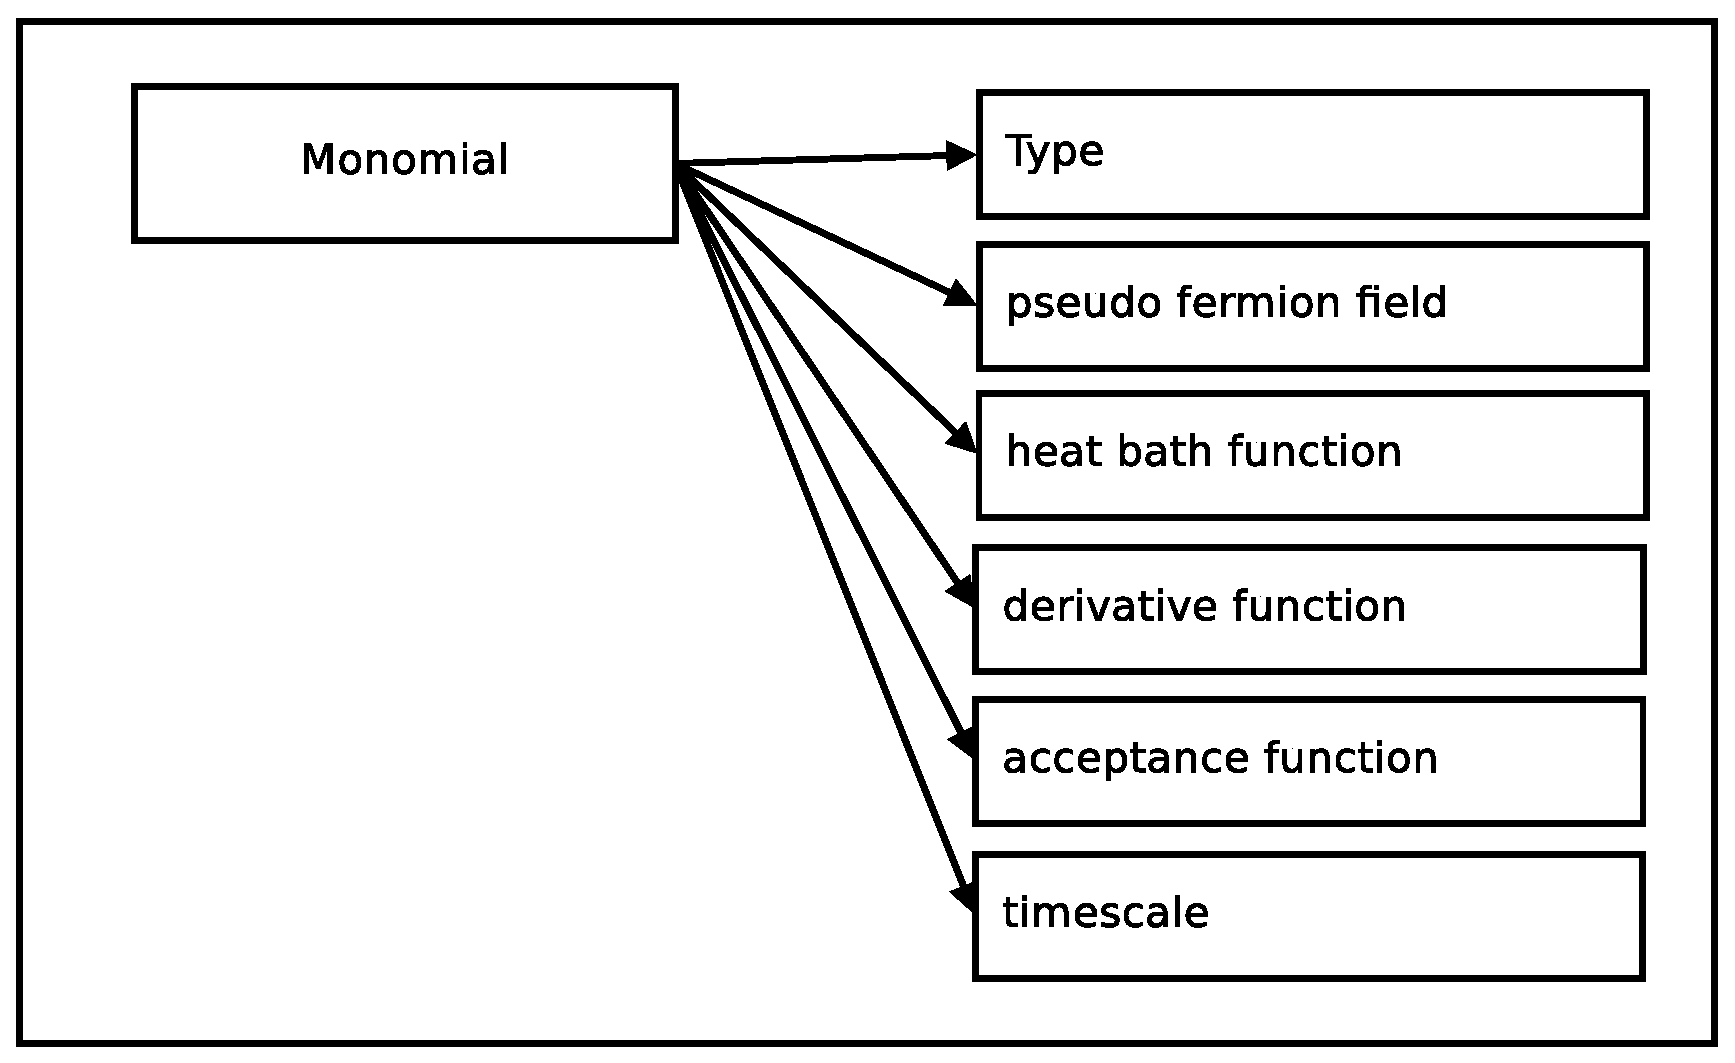
\includegraphics[width=0.7\linewidth]{monomial.eps}
  \caption{Data type monomial and its components}
  \label{fig:monomial}
\end{figure}

In addition for each monomial it needs to be known on which timescale
it should be integrated. The corresponding data type is sketched in
figure~\ref{fig:monomial}. The general definitions for this data type
can be found in the file {\ttfamily monomial.c}. 

There are several sorts of monomials implemented:
\begin{itemize}
\item {\ttfamily DET}: pseudo fermion representation of the (mass
  degenerate) simple determinant\\
  \[
  \det(Q^2(\kappa) + \mu^2)
  \]
\item {\ttfamily DETRATIO}: pseudo fermion representation of the
  determinant ratio\\
  \[
  \det(Q^2(\kappa) + \mu^2)/\det(Q^2(\kappa_2) + \mu_2^2)
  \]
\item {\ttfamily NDPOLY}: polynomial representation of the (possibly
  non-degenerate) doublet\\
  \[
  [\det(Q_{nd}(\bar\epsilon, \bar\mu)^2)]^{1/2}\, .
  \]
\item {\ttfamily GAUGE}:\\
  \[
  \frac{\beta}{3}\sum_x\left(  c_0\sum_{\substack{
        \mu,\nu=1\\1\leq\mu<\nu}}^4\{1-\re\tr(U^{1\times1}_{x,\mu,\nu})\}\Bigr. 
    \Bigl.\ +\ 
    c_1\sum_{\substack{\mu,\nu=1\\\mu\neq\nu}}^4\{1
    -\re\tr(U^{1\times2}_{x,\mu,\nu})\}\right)\,  ,
  \]
  The parameter $c_1$ can be set in the input file and
  $c_0=1-8c_1$. Note that $c_1=0$ corresponds to the Wilson plaquette
  gauge action. 
\end{itemize}
The corresponding specific functions are defined in the files
{\ttfamily det\_monomial.c}, {\ttfamily detratio\_monomial.c},
{\ttfamily ndpoly\_monomial.c} and {\ttfamily
  gauge\_monomial.c}. Additional monomials can easily be implemented
by providing the corresponding functions as discussed above.

\begin{algorithm}[t]
  \caption{integrate}
  \begin{algorithmic}[1]
    \REQUIRE $0 < n_\mathrm{ts}\leq N_\mathrm{ts}$, $\tau > 0$
    \STATE $\dtau = \tau/$noSteps[$n_\mathrm{ts}$]
    \FOR{$i$ = 0 to noSteps[$n_\mathrm{ts}$]}
    \IF{$n_\mathrm{ts}$ == $1$}
    \STATE updateGauge($\dtau$)
    \ELSE
    \STATE integrate($n_\mathrm{ts}-1$, $\dtau$)
    \ENDIF
    \STATE updateMomenta($\dtau$, monomialList[$n_\mathrm{ts}$])
    \ENDFOR
  \end{algorithmic}
  \label{alg:integrator}
\end{algorithm}

The integration scheme is implemented recursively, as exemplified in
algorithm~\ref{alg:integrator} for the leap-frog integration scheme
(where we skipped half steps for simlicity). The updateMomenta
function simply calls the derivative functions of all monomials
that are integrated on timescale $n_\mathrm{ts}$ and updates the
momenta $P$ according to the time step $\dtau$.

The recursive scheme for the integration can easily be extended to
more involved integration schemes. The details can be found in the
file {\ttfamily integrator.c}. We have implemented the leap-frog and
the second order minimal norm~\cite{Takaishi:2005tz} integrations
schemes. They are named in the input file as {\ttfamily LEAPFROG} and
{\ttfamily 2MN}, respectively. These two can be mixed on
different timescales. In addition we have implemented a position
version of the second order minimal norm integration scheme, denoted by
{\ttfamily 2MNPOSITION} in the input file. The latter must not be mixed with
the former two.

The MD update is summarised in
algorithm~\ref{alg:mdupdate}. It computes the initial and final
Hamiltonians and calls in between the integration function with the
total number of timescales $N_\mathrm{ts}$ and the total trajectory
length $\tau$.

\subsubsection{Reduced Precision in the MD Update}

As shortly discussed previously, as long as the integration in the MD
udpate is reversible and area preserving there is large freedom in
choosing the integration scheme, but also the operator: it is not
necessary to use the Dirac operator here, it can be any approximation
to it. This is only useful if the acceptance rate is not strongly
affected by such an approximation.

The code provides two possibilities to adapt the precision of the
Dirac operator used in the MD update: the first is to reduce the
precision in the inversions needed for the force computation. This
causes reduced iteration numbers needed for the integration of one
trajectory. The relevant input parameter is {\ttfamily
  ForcePrecision} available for each monomial. The precision needed in
the acceptance and/or heatbath step can be adjusted separately using
{\ttfamily AcceptancePrecision}. It is advisable to have the
acceptance precision always close to machine precision.


\begin{algorithm}[t]
  \caption{MD update}
  \begin{algorithmic}[1]
    \STATE $\mathcal{H}=\mathcal{H}'=0$
    \FOR{$i$ = 0 to $N_\mathrm{monomials}$} 
    \STATE $\mathcal{H}$ += monomial[$i$]$\rightarrow$heat-bath-function
    \ENDFOR

    \STATE integrate($N_\mathrm{ts}$, $\tau$)

    \FOR{$i$ = 0 to $N_\mathrm{monomials}$} 
    \STATE $\mathcal{H}'$ += monomial[$i$]$\rightarrow$acceptance-function
    \ENDFOR
    \STATE accept with probability $\min\{1, \exp(-\Delta\mathcal{H})\}$
  \end{algorithmic}
  \label{alg:mdupdate}
\end{algorithm}


The second possibility for influencing the Dirac operator is given by
the reduced precision Dirac operator described in
sub-section~\ref{sec:dirac}, which is switched on with the {\ttfamily
  UseSloppyPrecision} input parameter. The two possibilities can also
be used in parallel.

Note that one should always test for reversibility violations as
explained in sub-section \ref{sec:online}.

\subsubsection{Chronological Solver}

The idea of the chronological solver method (or similar methods
\cite{Brower:1994er}) is to optimize the initial guess for
the solution used in the solver. To this end the history of
$N_\mathrm{CSG}$ last solutions of the equation $M^2 \chi = \phi$ is
saved and then a linear combination of the fields $\chi_i$ with
coefficients $c_i$ is used as an initial guess for the next
inversion. $M$ stands for the operator to be inverted and has to be
replaced by the different ratios of operators used in this paper.

The coefficients $c_i$ are determined by solving
\begin{equation}
  \label{eq:chrono}
  \sum_i \chi_j^\dagger M^2 \chi_i c_i = \chi_j^\dagger \phi
\end{equation}
with respect to the coefficients $c_i$. This is equivalent to
minimising the functional that is minimised by the CG inverter
itself.

The downside of this method is that the reversibility violations
increase significantly by one or two orders of magnitude in the
Hamiltonian when the CSG is switched on and all other parameters are
kept fixed. Therefore one has to adjust the residues in the solvers,
which increases the number of matrix vector multiplications again.
Our experience is that the methods described in the previous
sub-section are more effective in particular in the context of
multiple time scale integration, because the CSG is most effective for
small values of $\dtau$.

The input parameters is the {\ttfamily CSGHistory} parameter
available for the relevant monomials. Setting it to zero means no
chronological solver, otherwise this parameter specifies the number of
last solutions $N_\mathrm{CSG}$ to be saved.

\subsection{Online Measurements}
\label{sec:online}

The HMC program includes the possibility to perform a certain number
of measurements after every trajectory \emph{online}, whether or not
the configuration is stored on disk. Some of those are performed per
default, namely all that are written to the output file {\ttfamily
  output.data}: 
\begin{enumerate}
\item the plaquette expectation value, defined as:
  \[
  \langle P\rangle = \frac{1}{6 V}\ \sum_{\substack{
        \mu,\nu=1\ 1\leq\mu<\nu}}^4\ \re\tr(U^{1\times1}_{x,\mu,\nu})\, ,
  \]
  where $V$ is the global lattice volume.
\item the rectangle expectation value, defined as:
  \[
  \langle R\rangle = \frac{1}{12V}\ \sum_{\substack{\mu,\nu=1\
      \mu\neq\nu}}^4\ 
    \re\tr(U^{1\times2}_{x,\mu,\nu})
  \]
\item $\Delta\mathcal{H} = \mathcal{H}'-\mathcal{H}$ and $\exp(-\Delta\mathcal{H})$.
\end{enumerate}
See the overview section for details about the {\ttfamily output.data}
file. These observables all come with no extra computational cost.

Optionally, other online measurements can be performed, which --
however -- need in general extra inversions of the Dirac
operator. First of all the computation of certain correlation
functions is implemented. They need \emph{one} extra inversion of the
Dirac operator, as discussed in Ref.~\cite{Boucaud:2008xu}, using the
one-end-trick. Define a stochastic source $\xi$ as follows
\begin{equation}
  \label{eq:source}
  \lim_{R\to\infty}[\xi_i^*\xi_j] = \delta_{ij},\quad
  \lim_{R\to\infty}[\xi_i\xi_j] = 0\, .
\end{equation}
Here $R$ labels the number of samples and $i$ all other degrees of
freedom. Then 
\begin{equation}
  \label{oneend}
  [\phi_i^{r*}\phi_j^r]_R = M_{ik}^{-1*}\cdot M_{jk}^{-1} +
  \textrm{noise}\, ,
\end{equation}
if $\phi$ was computed from
\[
\phi_j^r  = M^{-1}_{jk}\xi_k^r\, .
\]
Having in mind the $\gamma_5$-hermiticity property of the Wilson and
Wilson twisted mass Dirac propagator $G_{u,d}$, i.e.
\[
G_u(x,y) = \gamma_5 G_d(y,x)^\dagger \gamma_5
\]
it is clear that eq.~(\ref{oneend}) can be used to evaluate
\[
C_\pi(t) = \langle \tr[G_u(0,t)\gamma_5 G_d(t,0)\gamma_5]\rangle =
\langle \tr[G_u(0,t) G_u(0,t)^\dagger]\rangle
\]
with only one inversion. But, even if the one gamma structure at the
source is fixed to be $\gamma_5$ due to the $\gamma_5$-hermiticity
trick, we are still free to insert any $\gamma$-structure $\Gamma$ at the source,
i.e. we can evaluate any correlation function of the form
\[
C_{P\Gamma}(t) = \langle\tr[G_u(0,t) \gamma_5 G_d(t,0) \Gamma]\rangle
= \langle \tr[G_u(0,t) G_u(0,t)^\dagger\gamma_5\Gamma]\rangle\, .
\]
Useful combinations of correlation functions are $\langle P P\rangle$,
$\langle PA\rangle$ and $\langle PV\rangle$, with
\[
  P^\alpha = \bar\chi \gamma_5 \frac{\tau^\alpha}{2}\chi\, ,\quad
  V^\alpha_\mu = \bar\chi \gamma_\mu\frac{\tau^\alpha}{2}\chi\, ,\quad
  A^\alpha_\mu = \bar\chi \gamma_5\gamma_\mu\frac{\tau^\alpha}{2}\chi
\]
From $\langle P P\rangle$ one can extract the pseudo scalar mass, and
-- in the twisted mass case -- the pseudo scalar decay
constant. $\langle PA\rangle$ can be used together with $\langle P
P\rangle$ to extract the so called PCAC quark mass and $\langle
PV\rangle$ to measure the renormalisation constant $Z_\mathrm{V}$. For
details we refer the reader to Ref.~\cite{Boucaud:2008xu}.

These online measurements are controlled with the two following input
parameters: {\ttfamily PerformOnlineMeasurements} to switch them on or
off and to specify the frequency {\ttfamily OnlineMeasurementsFreq}. The three
correlation functions are saved in files named {\ttfamily
  onlinemeas.n}, where {\ttfamily n} is the trajectory number. Every
file contains five columns, specifying the type, the operator type and the
Euclidean time $t$. The last two columns are the values of the
correlation function itself, $C(t)$ and $C(-t)$, respectively. The
type is equal to $1$, $2$ or $6$ for the $\langle P P\rangle$, the
$\langle PA\rangle$ and the $\langle PV\rangle$ correlation
functions. The operator type is for online measurements always equal
to $1$ for local source and sink (no smearing of any kind), and the
time runs from $0$ to $T/2$. Hence, $C(-t)= C(T-t)$. $C(-0)$ and
$C(-T/2)$ are set to zero for convenience.

In addition to correlation functions also the minimal and the maximal
eigenvalues of the $(\gamma_5 D)^2$ can be measured.

An online measurement not related to physics, but related to the
algorithm are checks of reversibility violations. The HMC algorithm is
exact, if 
and only if the integration scheme is reversible. On a computer with
finite precision this is only guaranteed up to machine precision.
These violations can be estimated by integrating one trajectory
forward and then backward in Monte Carlo time. The difference
$\delta\Delta\mathcal{H}$ among
the original Hamiltonian $\mathcal{H}$ and the final one
$\mathcal{H}''$ after integrating back can serve as one measure for
those violations, another one is provided by the difference among the
original gauge field $U$ and the final one $U''$
\[
\delta\Delta U = \frac{1}{12V}
\sum_{x,\mu}\sum_{i,j} (U_{x,\mu}-U_{x,\mu}'')_{i,j}^2
\]
where we indicate with the $\delta\Delta$ that this is obtained after
integrating a trajectory forward and backward in time. The results for
$\delta\Delta \mathcal{H}$ and $\delta\Delta U$ are
stored in the file {\ttfamily return\_check.data}. The relevant input
parameters are {\ttfamily ReversibilityCheck} and {\ttfamily
  ReversibilityCheckInterval}.

\subsection{Iterative Solver and Eigensolver}

There are several iterative solvers implemented in the tmLQCD
package for solving 
\[
D\ \chi = \phi
\]
for $\chi$. The minimal residual (MR), the conjugate gradient (CG), the
conjugate gradient squared (CGS), the generalised minimal residual
(GMRES), the generalised conjugate residual and the stabilised
bi-conjugate gradient (BiCGstab). For details regarding these
algorithms we refer to Refs.~\cite{saad:2003a,meister:1999}.

For the {\ttfamily hmc\_tm} executable only the CG and the BiCGstab
solvers are available, while all the others can be used in the
{\ttfamily invert} executables. Most of them are both available with
and without even/odd preconditioning. For a performance comparison we
refer to Ref.~\cite{Chiarappa:2004ry,Chiarappa:2006hz}.

The stopping criterion is implemented in two ways: the first is an
absolute stopping criterion, i.e. the solver is stopped when the
squared norm of the residual vector (depending on the solver this
might be the iterated residual or the real residual) fulfills
\[
\|r\|^2 < \epsilon^2\, .
\]
The second is relative to the source vector, i.e.
\[
\frac{\|r\|^2}{\|\phi\|^2} < \epsilon^2\, .
\]
The value of $\epsilon^2$ and the choice of relative or absolute precision can be
influenced via input parameters.

The reduced precision Dirac operator, as discussed in sub-section
\ref{sec:dirac}, is available for the CG solver. In the CG solver the 
full precision Dirac operator is only required at the beginning of the
CG search, because the relative size of the contribution to the
resulting vector decreases with the number of iterations. Thus, as soon
as a certain precision is achieved in the CG algorithm we can switch to
the reduced precision Dirac operator without spoiling the precision of
the final result. We switch to the lower precision operator 
at a precision of $\sqrt{\epsilon}$ in the CG search, when aiming for a
final precision of $\epsilon < 1$.

The eigensolver used to compute the eigenvalues (and vectors) of
$(\gamma_5 D)^2$ is the so called Jacobi-Davidson 
method~\cite{Sleijpen:1996aa,Geus:2002}. For a discussion for the
application of this algorithm to lattice QCD we refer again to
Ref.~\cite{Chiarappa:2004ry,Chiarappa:2006hz}. 

All solver related files can be found in the sub-directory {\ttfamily
  solver}. Note that there are a few more solvers implemented which
are, however, in an experimental status.

\subsection{Stout Smearing}

Smearing techniques have become an important tool to reduce
ultraviolet fluctuations in the gauge fields. One of those techniques,
coming with the advantage of being usable in the MD update, is usually
called stout smearing~\cite{Morningstar:2003gk}. 

The $(n+1)^{\rm th}$ level of stout smeared gauge links is obtained iteratively
from the $n^{\rm th}$ level by
\begin{equation*}
  U_\mu^{(n+1)}(x)\;=\;e^{i\,Q_\mu^{(n)}(x)}\,U_\mu^{(n)}(x).
\end{equation*}
We refer to the unsmeared (``thin'') gauge field as $U_\mu\equiv
U_\mu^{(0)}$.
The ${\rm SU}(3)$ matrices $Q_\mu$ are defined via the staples $C_\mu$:
\begin{eqnarray}
  Q_\mu^{(n)}(x) &=& \frac{i}2\Big[U^{(n)}_\mu(x){C_\mu^{(n)}}^\dagger(x)
  - {\mathrm{h.c.}}\Big]\,-\,\frac{i}{6}\tr\Big[U^{(n)}_\mu(x){C_\mu^{(n)}}^\dagger(x)
  - {\mathrm{h.c.}}\Big]\,,\nonumber\\
  C_\mu^{(n)} &=& \sum_{\nu\neq\mu}\,\rho_{\mu\nu}\,
  \Big(U_\nu^{(n)}(x)U_\mu^{(n)}(x+\hat\nu){U_\nu^{(n)}}^\dagger(x+\hat\mu)
  \nonumber\\
  && \;\;\;
  +{U_\nu^{(n)}}^\dagger(x-\hat\nu)U_\mu^{(n)}(x-\hat\nu)U_\nu^{(n)}(x-\hat\nu+\hat\mu)
  \Big)\,,\nonumber
\end{eqnarray}
where in general $\rho_{\mu\nu}$ is the smearing matrix.
In the tmLQCD package we have only implemented isotropic $4$-dimensional
smearing, i.e., $\rho_{\mu\nu}=\rho$.

Currently stout smearing is only implemented for the {\ttfamily
  invert} executables. I.e. the gauge field can be stout smeared at
the beginning of an inversion. The input parameters are {\ttfamily
  UseStoutSmearing}, {\ttfamily StoutRho} and {\ttfamily
  StoutNoIterations}. 

\subsection{Random Number Generator}

The random number generator used in the code is the one proposed by
Martin L{\"u}scher and usually known under the name
RANLUX~\cite{Luscher:1993dy}. A single and double precision
implementation was made available by the author under the GNU General
Public License and can be downloaded~\cite{Luscher:ranluxweb}. For
convenience it is also included in the tmLQCD package.


\endinput

%%% Local Variables: 
%%% mode: latex
%%% TeX-master: "main"
%%% End: 
